\chapter{Our work}
\label{kap:kap3}

In this chapter, we shall look into our new enhancements to the existing
implementation of RRR. We shall at first propose a new block encoding
method. Then, we shall show how we can exploit the assumtions about the
share of ones in the bit sequence.  

\section{Block encoding}

As we already discussed in section~\ref{section:compressed_bv}, there are to
the best of our knowledge two widely used methods to encode and decode the
block in RRR. The main disadvantage of the table decoding method is the big space
overhead that it is using and the inability to reasonably support a longer blocks
in practice because of the huge table sizes for bigger block length. On the
other hand, the on-the-fly decoding method can be used to support a bigger block size
with the downside of longer encoding and decoding times. We shall now propose
new method of encoding and decoding the blocks. The main objective of the new method is
to create an alternative to the previous methods that enables a use of longer blocks
while not hurting the runtime so significantly.

The main idea behind our solution is to use a divide-and-conquer approach to break
the problem of finding the order of the block $B$ along the class $c$ to finding the order
of the several smaller blocks. This will enable us to use the table method to solve the
smaller subproblems. To facilitate our solution, we need to alter the respective order of
the blocks along the same class. We want to note that we also use the number of ones to
identify the class of block. Both previous solutions used the lexicographical ordering
for the blocks that shared the same class. In our solution, every block $B$ will be thought
of as two smaller blocks of half the size, namely $B_1$ and $B_2$. We shall at first sort the
big block $B$ by the pair $(c_1, c_2)$ and then, subsequently by $B_1$ and $B_2$ where $c_1$
and $c_2$ are the respective classes of the smaller blocks $B_1$ and $B_2$. Note that the
original lexicographical ordering can be rephrased in the context of sub-blocks as sorting
at first by $B_1$ and then by $B_2$. The example of the ordering for concrete block length
and one class is shown on Figure~\ref{obr:lexicographicalVsUs}.

\begin{figure}
	\centerline{
        \begin{tabular}{l c l}
            Offset  &   Block       & $(c_1, c_2)$\\
        \hline
            \small 0&   \tt 000 011 & \multirow{3}{*}{$(0, 2)$}\\
            \small 1&   \tt 000 101 & \\
            \small 2&   \tt 000 110 & \\
        \hline
            \small 3&   \tt 001 001 & \multirow{5}{*}{$(1, 1)$}\\
            \small 4&   \tt 001 010 &\\
            \small 5&   \tt 001 100 &\\
            \small 6&   \tt 010 001 &\\
            \small 7&   \tt 010 010 &\\
        \end{tabular}
        \hspace{3em}
        \begin{tabular}{l c l}
            \small 8&   \tt 010 100 & \multirow{4}{*}{$(1, 1)$}\\
            \small 9&   \tt 100 001 &\\
            \small 10&  \tt 100 010 &\\
            \small 11&  \tt 100 100 & \\
        \hline
            \small 12&  \tt 011 000 & \multirow{3}{*}{$(2, 0)$}\\
            \small 13&  \tt 101 000 &\\
            \small 14&  \tt 110 000 &\\
        \end{tabular}
	}
	\caption[TODO]{
        Example of the new ordering for the block length $b=6$ and class $c=2$.
        Every block is divided into two sub-blocks of size 3. Note the differences to the
        lexicographical ordering. Block {\tt 011 000} on offset 12 is preceded by lexicographicaly
        greater blocks {\tt 100 001}, {\tt 100 010} and {\tt 100 100} as it has bigger number of ones
        in the first sub-block.
    }
	\label{obr:lexicographicalVsUs}
\end{figure}

We shall now demonstrate how we use this new ordering and that it is convenient to encode and
decode $B$ in a divide and conquer manner.

\paragraph{Encoding}

Before providing the general encoding stratedy, we shall demonstrate the encoding with
simple example and then generalize the ideas behind the process. Imagine encoding
block {\tt 100 010}. We can see that the class of this block is 2 as there are two ones in
the block. Obtaining the offset is more complicated. We will proceed by enumerating the
number of smaller blocks in the class $c=2$. There are three types of blocks preceding
block {\tt 100 010} along its class. These are:

\begin{itemize}
    \item Blocks with the smaller number of ones in the first sub-block.
    (There are 3 such blocks -- those beginning with {\tt 000}.)
    \item Blocks with the same number of ones in the first sub-block, but smaller first sub-block.
    (There are 6 blocks with this property -- those beginning with {\tt 010} or {\tt 001}.)
    \item Blocks with the same first sub-block, but smaller second sub-block.
    (There is 1 such block, namely {\tt 100 001}.)
\end{itemize}

Summing up, we get that there are 10 blocks preceding {\tt 100 010} so it has the offset $o$
equal to 10. Together with class we would encode this block as a pair $(2, 10)$.

In general, consider a block $B$ of length $b$. The first step is to obtain
$c$ -- the class of the block. This can be done by counting ones in $B$. We
then get that $$c=\#_1(B)$$. To obtain the sequence number $o$ of $B$, we shall
count the number of blocks preceding $B$ along the class $c$. There are three
types of blocks preceding $B$:

\begin{enumerate}
    \item Blocks with the first sub-block having smaller class than $B_1$.
    \label{chapter3:encoding:1}
    \item Blocks with the first sub-block being of the same class as is $B_1$
    but with smaller first sub-block. \label{chapter3:encoding:2}
    \item Blocks with the same first sub-block but smaller second sub-block.
    \label{chapter3:encoding:3}
\end{enumerate}

Formalizing this, we shall write $B\prec_X B'$ if blocks $B$ and $B'$ are of
the same length, class and $B$ precedes $B'$ in ordering $X$. We shall
write $B\prec_{\Lex} B'$ if $B$ preceeds $B'$ in lexicographical ordering.
To formally define our new proposed ordering $P$, we shall write that
\begin{align*}
    B\prec_P B' \iff
    &[\#_1(B_1) < \#_1(B_1')] \\
    &\lor [(\#_1(B_1) = \#_1(B_1')) \land B_1 < B_1']\\
    &\lor [B_1 = B_1' \land B_2 < B_2']
\end{align*}
where $B=B_1B_2$ and $B'=B_1'B_2'$.

The number of blocks in group~\ref{chapter3:encoding:1} is equal to
$$\sum_{i=0}^{c_1-1} {15\choose i} {15\choose c-i}$$ where $i$ denotes the number
of ones in the first block. Terms ${15\choose i}$ and ${15\choose c-i}$ denote the
number of blocks if there is $i$-ones in the first sub-block and the rest $c-i$ ones
in the second sub-block.

The number of blocks in group~\ref{chapter3:encoding:2} is equal to the number of blocks that
share classes of sub-blocks, but are smaller than $B$. Number of these blocks is $o_1\times {15\choose c_1}$.
The number of blocks in group~\ref{chapter3:encoding:3} is equal to the number of blocks smaller 
than $B_2$. This is identical to the offset $o_2$. Note that to obtain the offset of $B$
we need to have the encoding of the blocks $B_1$ and $B_2$. These are two pairs of numbers
$(c_1, o_1)$ and $(c_2, o_2)$ that can be computed recursively.

\paragraph{Decoding}

Decoding is a process of obtaining block representation $B$ from the encoded
representation $(c, o)$. We would like to use our sub-routines for the blocks
of size $b/2$. However, to use these we need to find the classes and offsets of
the smaller blocks. Namely, we need to find what the pairs $(c_1, o_1)$ and
$(c_2, o_2)$ are. We shall again present this process on a example and decode
the block from previous encoding example {\tt 100 010} encoded as $(2, 10)$.
To obtain the number of ones in the first sub-block only from the offset of the
block, we can look into the table and see that there are 3 blocks with zero ones
in the first sub-block. As the offset of our block is ten, we need to look for this
block between blocks with more than 0 ones. There are 9 blocks with one 1 in the first
sub-block. As $3+9$ is bigger than 10, we discovered that the number of ones in the
first block is 1 and it follows that the number of ones in the second sub-block is
also 1 as we know the total number of ones in the block. There are 9 blocks with
this exact same property, the smallest one being {\tt 001 001} and largest one
{\tt 100 100}. We now focus on identifying what is the offset of the first and second
sub-block. There are ${3 \choose 1} = 3$ possibilities (namely {\tt 001}, {\tt 010},
{\tt 100}) how the first and also the second block may look. Blocks are sorted according
to the first sub-block and then second sub-block. As all the combinations of the first
block and second block are possible, all possible second sub-blocks will be cyclically
repeating again and again with the increasing first sub-block. Cycle through
the sub-blocks will be of length 3 (number of possible second sub-blocks) and will repeat
3 times (number of possible first sub-blocks). Along these ordering of 9 blocks we are
looking for the 7th. The first sub-block will change exactly 2 times to {\tt 100} and on the
7th iteration through this ordering the second sub-block is {\tt 010}.

% TODO: finish this

In general,

pairs we need to find out what are the number of blocks in the groups \ref{chapter3:encoding:1},
\ref{chapter3:encoding:2} and \ref{chapter3:encoding:3}. To simplify, we will define $C_i$ to be a 
number of blocks of length $b$ with less than or equal number of ones in the first block than $i$.
We then compute the values of $C_i$ for every $i$ ($0\leq i\leq c$). Note that from the definition
$C_i = \sum_{j=0}^{i} {15 \choose j} {15 \choose c-j}$. To found $c_1$ we need to basically find the
biggest $C_{max}$ such that $o<C_{max}$. After finding it, we know that $c_1 = max+1$ and that
$c_2 = c - c_1$. Problem is that number of elements from group~\ref{chapter3:encoding:2} and
\ref{chapter3:encoding:3} is in total equal to $C_{max}-o$ but we do not know the exact number
of the elements in the respective group yet. However, we know the number of ones in each sub-block,
so we need to just get a respective $o_1$ and $o_2$ to again use our table decoding subroutine. We
know that $C_{max}-o = {15 \choose c_2} + x$.

\paragraph{Combining encoding methods}

Our proposed method can be used to obtain the encoding and decoding scheme for block size $b$
using only the scheme for block size of $b/2$. As we already mentioned in
subsection~\ref{subsection:block_size}, most of the implementations of RRR choose the size
of the block in the form of $2^k-1$ as the number of ones is the power of two and it fits
exactly into $k$ bits. This is not very convenient as combining two solutions of size
$2^k-1$ combined together give us only $2(2^k-1)$ that is one bit short of a practically
usable size. To overcome this, we need to extend the block by one bit. To do this, we
shall once again alter the order of the blocks along the same class. Let us now look on
an example how to obtain blocks of length 5 and class 3. There will be two types of blocks
in this class. One of the form {\tt 0xxxx} and second of the form {\tt 1xxxx}. There are
${4\choose 3}$ ways how to distribute 3 ones along the four places so there will be exactly
4 blocks starting with 0 and ${4\choose 2}$ blocks starting with one. Blocks starting with
zero will continue with all the possible blocks of length 4 and class 3. These blocks will
can come in any valid ordering but we can already use our newly devised technique of block
encoding. The complete order of the blocks in this example appears in Fig.~\ref{obr:bitExtension}.

\begin{figure}
	\centerline{
        \begin{tabular}{l c}
            Offset  &   Block      \\
        \hline
            \small 0&   \tt 0 0111 \\
            \small 1&   \tt 0 1011 \\
            \small 2&   \tt 0 1101 \\
            \small 3&   \tt 0 1110 \\
        \end{tabular}
        \hspace{4em}
        \begin{tabular}{l c}
            \small 4&   \tt 1 0011 \\
            \small 5&   \tt 1 0101 \\
            \small 6&   \tt 1 0110 \\
            \small 7&   \tt 1 1001 \\
            \small 8&   \tt 1 1010 \\
            \small 9&   \tt 1 1100 \\
        \end{tabular}
	}
	\caption[TODO]{
        Example of bit extension of block length 4 to length 5. Table shows the
        order of blocks along the class $c=3$. These are primarily sorted
        by the first expansion bit. Blocks with the same value of expansion
        bit are sorted according to the method we introduces previously.
    }
	\label{obr:bitExtension}
\end{figure}

\section{Hybrid encoding}

Let us now consider a randomly generated bit sequence $B$ of length $n$ with the $p\%$
of ones in it. We shall make some general observations about the distribution of block
classes of this bit sequence. If we consider a block size $b$ then the random variable
$X$ denoting number of ones in the block follows a binomial distribution:
            $$X \sim Bin(b,p)$$.

\begin{figure}
	\centerline{
		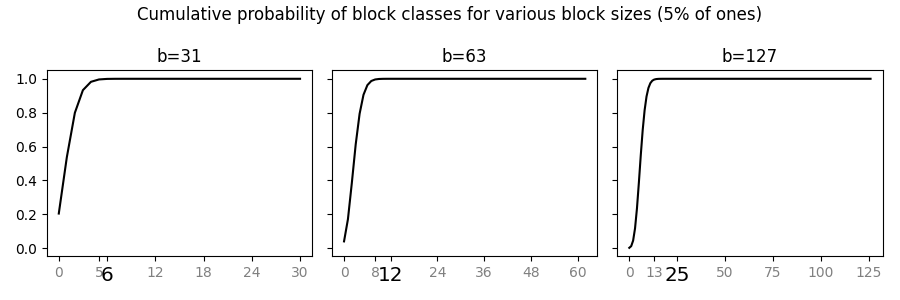
\includegraphics[width=\textwidth]{images/hybrid_encoding_motivation}
	}
	\caption[TODO]{On these 3 graphs, we can see the cummulative distribution
    of blocks classes for the block sizes of 31, 63, 127. The frequency of ones is
    fixed to 5\%. Note the marked classes on x-axis. Numbers 6, 12 and
    25 mark the place up to which 99\% of probability distribution lies for
    the block sizes 31, 63, 127 respectively.
	}
	\label{obr:hybridEncodingDistribution}
\end{figure}

RRR saves most of the memory on the sparse blocks, those with small number of
As we may observe on the Fig.~TODO, the probability of dense blocks in the sequence
containing only 5\% of ones is really small. Even in very long sequences, dense blocks
will be represented very sparse. This leads us to a solution that we called a
\textit{hybrid encoding}. Idea of this encoding is to encode 